\textsc{}% Chapter X

\chapter{Infection of murine macrophages by \textit{Salmonella}} % Chapter title

\label{ch:02-03} % For referencing the chapter elsewhere, use \autoref{ch:name} 

%----------------------------------------------------------------------------------------

In the former chapter, we presented the investigation of the infection process of a natural host by a bacterial pathogen. In this chapter, we investigate the opportunistic infection of mammalian macrophages by \textit{Salmonella enterica} through the prism of genome folding. Notably whether, and how \textit{S. enterica} infection affects the chromatin of its eukaryotic host. Much like \textit{Legionella}, \textit{Salmonella} manipulates its host cell's defense and signalling to promote its own survival in their cytoplasm \cite{larockSalmonellaeInteractionsHost2015}. Using a mouse \acrfull{BMM} model, we measured changes in chromatin architecture, accessibility and gene expression in different infection conditions and timepoints to explore the potential epigenetic deregulations happening during this process.

In the case of \textit{A. castellanii}, infection involved an unicellular host. Here, infection takes place in mammalian cells, whose much larger genomes have an intertwined, complex tridimensional organization. Notably, they are segmented into active and inactive compartments, and they contain long-range regulatory elements organized into chromatin domains and exhibiting cell type specificity \cite{schmittCompendiumChromatinContact2016}.

Here we focus on bone marrow-derived macrophages. These cells originate from hematopoietic stem cells and go through a complex differentiation process (Fig. \ref{fig:02-03:macrophage}a). After differentiation, they retain a strong plasticity and can be activated by cues in their environment to become "polarized" into one of two main activation states (Fig. \ref{fig:02-03:macrophage}b). M1 macrophages secrete high amounts of cytokines and promote inflammation, while M2 macrophages suppress immune response and focus on tissue repair \cite{ahmedM1M2Macrophages2020}. Together with neutrophils, M1 Macrophages are first responders to infection and act as key modulators and effectors cells during the immune response. During a bacterial infection, they will indeed phagocytose bacterial cells and initiate adaptive immunity by activating T cells through antigen presentation via the Major Histocompatibility Complex II (MHC-II). Additionally, they release cytokines and chemokines, which promote inflammation and further recruitment of other immune cells, and secrete anti-microbial molecules to destroy infectious cells. However, in the case of a prolonged infection, this strong immune reaction can have detrimental outcomes to the host and result in organ damages, or even lethal shock \cite{magesGenomewideAnalysisLPS2008}. This overstimulation is avoided by a process known as endotoxin- or LPS-tolerance. This state of reduced immune response is triggered by continuous exposure to lipopolysaccharides exposed on the bacterial cell surface and skews the macrophage population towards M2 polarization \cite{portaToleranceM2Alternative2009}. LPS-tolerance must also be tightly balanced, as suppressed immunity can lead to secondary infection or even sepsis. Such regulation is known to involve a combination of signalling and gene-specific chromatin changes through histone modifications \cite{aungLPSRegulatesProinflammatory2006}.

 Throughout the next sections, we describe an ongoing investigation, done in collaboration with the laboratory of Sophie Helaine at Harvard Medical School and her postdoc Peter W. Hill currently at Imperial College, of changes in chromosome conformation in macrophages following infection by \textit{Salmonella}. As we will focus on changes happening during late infection, LPS-tolerance is especially relevant to the understanding of this chapter.

\begin{figure}[htb]
    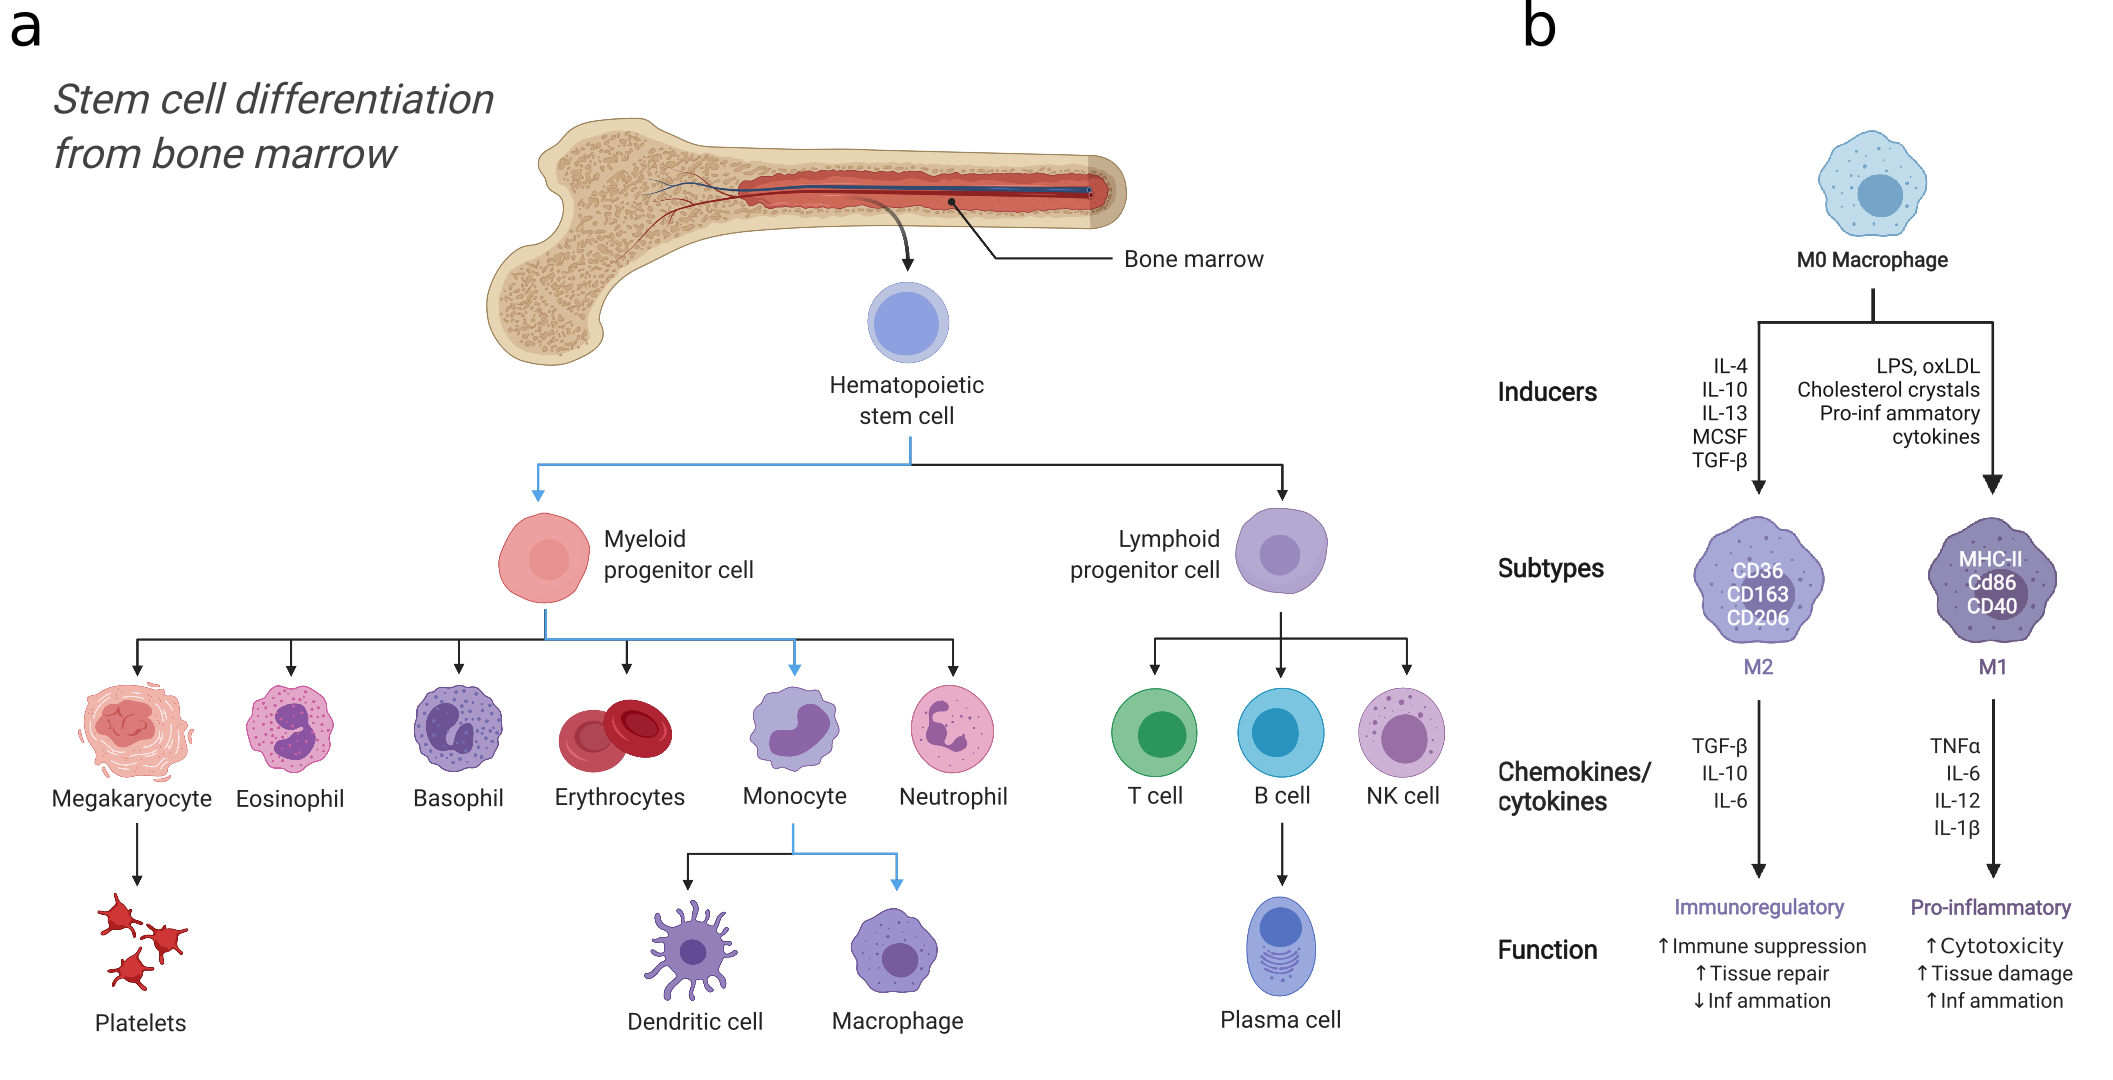
\includegraphics[width=\textwidth]{Parts/Part02/gfx/macrophage_differentiation.png}
    \caption[Macrophage differentiation.]{Macrophage differentiation from hematopoietic stem cells. \textbf{a:} Cellular differentiation pathway leading from bone marrow stem cells to macrophages \textbf{b:} Macrophage polarization from M0 to M1 (pro-inflammatory) or M2 (anti-inflammatory) macrophages. For either forms, molecules associated with induction of polarization, surface exposure and secretion are listed, as well as its functions. Adapted from "Stem cell differentiation from bone marrow" and "Macrophage subtypes in atherosclerosis", by BioRender.com (2020). Retrieved from https://app.biorender.com/biorender-templates}
    \label{fig:02-03:macrophage}
\end{figure}


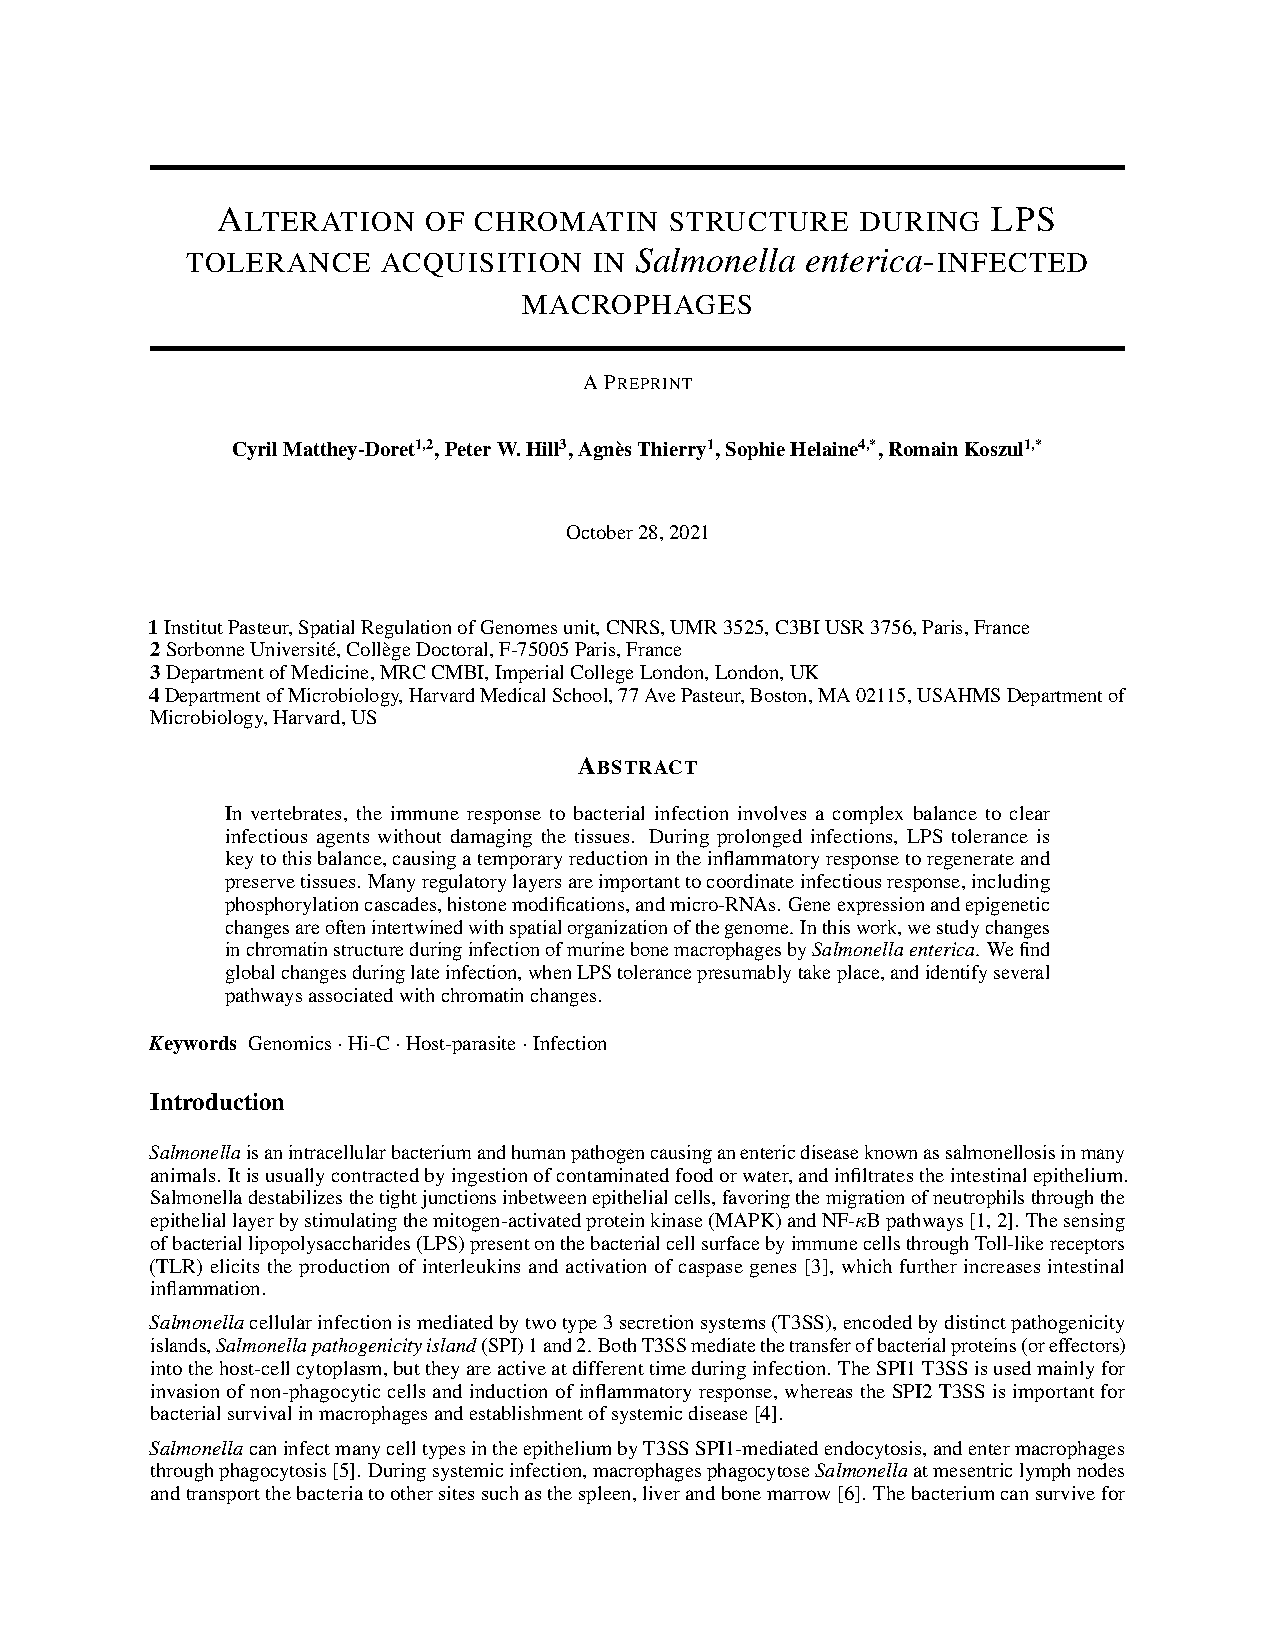
\includepdf[pages=-,addtotoc={
     1,section,1,Alteration of chromatin structure in macrophages during infection by \textit{Salmonella},p1,
     1,subsection,2,Introduction,sec:02-03:se-int,
     2,subsection,2,Results,sec:02-03:se-res,
     4,subsection,2,Discussion,sec:02-03:se-dis,
     7,subsection,2,Methods,sec:02-03:se-met,
     12,subsection,2,Supplementary figures,sec:02-03:se-sup}]
     {Publications/mouse_salmonella_manuscript.pdf}    